\section{Benchmarking Implementation} 

The experiments were run on IBM Q Boeblingen hardware on days 01/23-31/2021 for three times a day such that 
\begin{itemize}
    \item Run 1 of the day was run around 6:30 am after the first calibration of the device, 
    \item Run 2 of the day was run around 3:00 pm which is about 12 hours after the first calibration of the device,  
    \item Run 3 of the day started around 8:30 pm after second calibration of the device.
\end{itemize} 
We chose 3 qubit layouts to run the cycle benchmarking protocol to decide about which qubit layout provides the best performance for the open boundary conditions (OBC) Ising model Hamiltonian time evolution using Trotterization. These qubit layouts are
\begin{itemize}
    \item $[q_0,q_1,q_2,q_3]=[0,1,2,3]$ which is a layout in the upper left corner of the device,
    \item $[q_0,q_1,q_2,q_3]=[6,7,11,12]$ which is a layout in the middle of the device,
    \item $[q_0,q_1,q_2,q_3]=[16,17,18,19]$ which is a layout in the lower right corner of the device.
\end{itemize}



The experiments were run IBM Q Boeblingen device which has the qubit layout as seen in Fig.~\ref{fig:BoeblingenLayout}. 
\begin{figure}[ht!]
    % \centering
    % \includegraphics[width=2.2\columnwidth]{final_plot.pdf}
    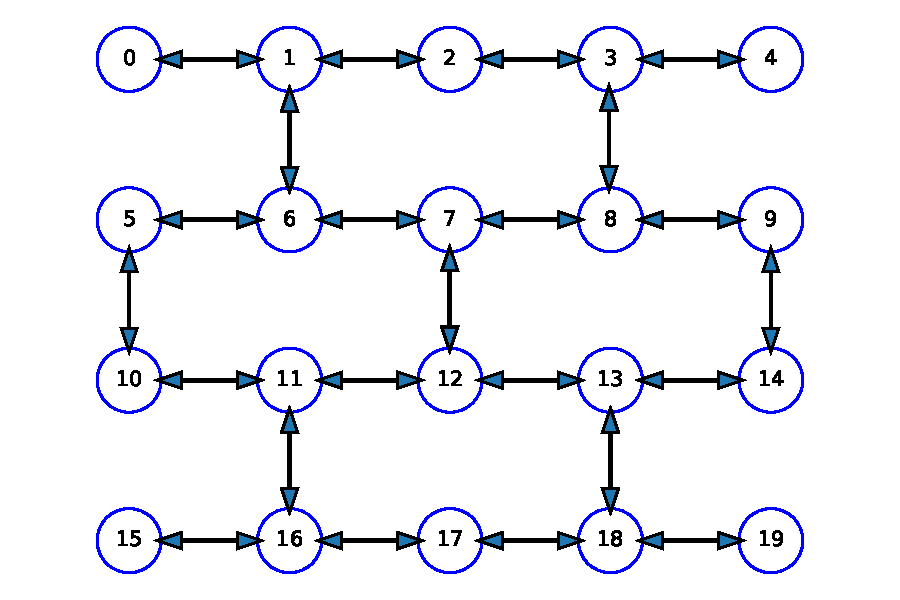
\includegraphics[scale=0.45]{QubitLayoutBoeblingen.pdf}
    \caption{IBM Q Boeblingen device qubit layout.}
    \label{fig:BoeblingenLayout}
\end{figure}


\subsection{Benchmarking Measurements}